\chapter{Orbitais moleculares das moléculas diatômicas}\label{ch:b2:diatomic-mos}

Despeje oxigênio líquido entre os polos de um ímã potente e ele é desviado
para o lado; o nitrogênio líquido cai em linha reta. A molécula de oxigênio
tem elétrons desemparelhados, que um campo magnético atrai. Sua estrutura de
Lewis, \ce{O=O}, com todos os elétrons emparelhados, não consegue dizer isso.
Os \omterm{def:b2:diatomic-mos:lcao}{orbitais moleculares}, construídos a partir dos orbitais atômicos do
capítulo anterior, colocam cada elétron de uma molécula em um nível próprio:
eles explicam o magnetismo do oxigênio, a força e o comprimento das ligações
e as energias necessárias para ionizar as moléculas --- e preparam o terreno
para a reatividade dos capítulos seguintes.

\begin{recall}
\Cref{ch:b2:atomic-orbitals}: os orbitais atômicos, suas formas, sinais e
energias. O volume do 1.º ano: estruturas de Lewis, ligações $\sigma$ e $\pi$
como noções descritivas, a hibridização e seus limites, elétrons
desemparelhados e radicais.
\end{recall}

\begin{omfigure}
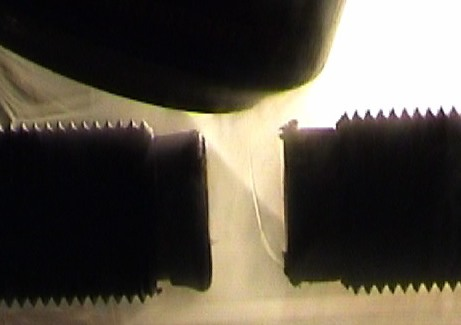
\includegraphics[width=0.42\linewidth]{images/book3/liquid-oxygen.jpg}

{\small Um fino filete de oxigênio líquido, que cai entre os polos de um ímã
potente, é atraído por eles e fica suspenso como uma ponte: a molécula é
\omterm{def:b2:diatomic-mos:magnetism}{paramagnética}. (Fotografia: Pieter Kuiper, domínio público, Wikimedia Commons.)}
\end{omfigure}

\section{O método CLOA}

\begin{definition}[Orbital molecular]\label{def:b2:diatomic-mos:lcao}
Um \emph{orbital molecular}\index{orbital molecular} é a \omterm{def:b2:atomic-orbitals:wavefunction}{função de onda} de um
elétron em uma molécula, estendida sobre todos os seus núcleos. No método
\emph{CLOA}\index{CLOA} (combinação linear de orbitais atômicos), ele é escrito
como uma soma de orbitais atômicos dos átomos, $\psi = \sum_i c_i\varphi_i$, com
coeficientes escolhidos para tornar a energia a mais baixa possível.
\end{definition}

Para dois átomos A e B, cada um trazendo um orbital, $\psi = c_A\varphi_A + c_B\varphi_B$.
A energia de um elétron em $\psi$, minimizada em relação aos coeficientes,
faz intervir três números.

\begin{definition}[As integrais do método CLOA]\label{def:b2:diatomic-mos:integrals}
Para dois orbitais atômicos reais $\varphi_A$, $\varphi_B$ e o operador energia $\hat H$
de um elétron na molécula:
\begin{itemize}
  \item a \emph{integral de sobreposição}\index{integral de sobreposicao@integral de sobreposição} $S = \int\varphi_A\varphi_B\,dV$
        mede o quanto os dois orbitais ocupam a mesma região ($S = 1$ para
        orbitais idênticos superpostos);
  \item a \emph{integral de Coulomb}\index{integral de Coulomb} $\alpha_A = \int\varphi_A\hat
        H\varphi_A\,dV$ é a energia de um elétron em $\varphi_A$ dentro da molécula,
        próxima da \omterm{def:b2:atomic-orbitals:orbital-energy}{energia orbital} atômica;
  \item a \emph{integral de ressonância}\index{integral de ressonancia@integral de ressonância} $\beta = \int\varphi_A\hat
        H\varphi_B\,dV$, negativa, mede o acoplamento dos dois orbitais.
\end{itemize}
As energias $E$ dos \omterm{def:b2:diatomic-mos:lcao}{orbitais moleculares} são as raízes do \emph{determinante
secular}\index{determinante secular}
\[
  \begin{vmatrix} \alpha_A - E & \beta - ES \\ \beta - ES & \alpha_B - E \end{vmatrix} = 0 .
\]
\end{definition}

O determinante vem da minimização de $E = \int\psi\hat H\psi\,dV/\int\psi^2\,dV$
em relação a $c_A$ e $c_B$: as duas condições $\partial E/\partial c_A =
\partial E/\partial c_B = 0$ formam um sistema linear homogêneo, que só tem
solução não nula quando seu determinante se anula. Essa etapa variacional é
admitida aqui.

\begin{theorem}[Dois orbitais idênticos]\label{thm:b2:diatomic-mos:homonuclear}
Para $\alpha_A = \alpha_B = \alpha$, os dois \omterm{def:b2:diatomic-mos:lcao}{orbitais moleculares} são
\[
  E_+ = \frac{\alpha + \beta}{1 + S}, \quad \psi_+ = \frac{\varphi_A + \varphi_B}{\sqrt{2(1 + S)}} ;
  \qquad
  E_- = \frac{\alpha - \beta}{1 - S}, \quad \psi_- = \frac{\varphi_A - \varphi_B}{\sqrt{2(1 - S)}} .
\]
\end{theorem}

\begin{proof}
O determinante dá $(\alpha - E)^2 = (\beta - ES)^2$, logo $\alpha - E = \pm(\beta - ES)$.
Com o sinal mais, $E(1 + S) = \alpha + \beta$; com o sinal menos, $E(1 - S) = \alpha
- \beta$. De volta ao sistema linear, $(\alpha - E)c_A + (\beta - ES)c_B = 0$ dá $c_B
= c_A$ para $E_+$ e $c_B = -c_A$ para $E_-$. Normalização: $\int(\varphi_A \pm
\varphi_B)^2\,dV = 2 \pm 2S$.
\end{proof}

\begin{definition}[Orbitais ligantes e antiligantes]\label{def:b2:diatomic-mos:bonding}
Um \emph{orbital ligante}\index{orbital ligante} fica abaixo dos orbitais
atômicos que o formam: sua densidade eletrônica se acumula entre os núcleos.
Um \emph{orbital antiligante}\index{orbital antiligante} fica acima deles e
tem um plano nodal entre os núcleos. Um \emph{orbital não ligante}\index{orbital nao ligante@orbital não ligante}
conserva a energia do orbital atômico, que não encontra parceiro com que se
combinar.
\end{definition}

\begin{proposition}[O orbital antiligante sobe mais]\label{prop:b2:diatomic-mos:asymmetry}
Para $S > 0$, o nível antiligante é elevado acima de $\alpha$ mais do que o
nível ligante é abaixado abaixo dele.
\end{proposition}

\begin{proof}
$E_+ - \alpha = (\beta - \alpha S)/(1 + S)$ e $E_- - \alpha = -(\beta - \alpha S)/(1 - S)$.
O numerador $\beta - \alpha S$ é negativo (o acoplamento domina), e $1 - S < 1
+ S$: o segundo deslocamento é maior em valor absoluto.
\end{proof}

Com dois elétrons, como em \ce{H2}, ambos entram em $\psi_+$, e a molécula é
mais estável que os átomos separados. Com quatro, como em \ce{He2}, dois
precisam entrar em $\psi_-$, o que custa mais do que $\psi_+$ ganha: \ce{He2}
não é ligada.

\begin{omfigure}
\begin{MOdiagram}[names, labels]
  \atom[H]{left}{ 1s = {0;up} }
  \atom[H]{right}{ 1s = {0;up} }
  \molecule[\ce{H2}]{ 1sMO = {.75;pair} }
\end{MOdiagram}
\hspace{1.5cm}
\begin{MOdiagram}[names, labels]
  \atom[He]{left}{ 1s = {0;pair} }
  \atom[He]{right}{ 1s = {0;pair} }
  \molecule[\ce{He2}]{ 1sMO = {.75;pair,pair} }
\end{MOdiagram}

{\small Diagramas de \omterm{def:b2:diatomic-mos:lcao}{orbitais moleculares} de \ce{H2} (\omterm{def:b2:diatomic-mos:bond-order}{ordem de ligação} 1) e de
\ce{He2} (\omterm{def:b2:diatomic-mos:bond-order}{ordem de ligação} 0, não ligada). Cada caixa é um nível que comporta no
máximo dois elétrons de spins opostos; linhas tracejadas ligam cada \omterm{def:b2:diatomic-mos:lcao}{orbital
molecular} aos orbitais atômicos a partir dos quais ele é construído.}
\end{omfigure}

\section{Sobreposição e simetria}

\begin{definition}[Orbitais $\sigma$ e $\pi$]\label{def:b2:diatomic-mos:sigma-pi}
Um \emph{orbital $\sigma$}\index{orbital sigma@orbital $\sigma$} de uma molécula linear não muda por
nenhuma rotação em torno do eixo molecular: ele não tem plano nodal que
contenha o eixo. Um \emph{orbital $\pi$}\index{orbital pi@orbital $\pi$} muda de sinal por
uma rotação de $180^\circ$ em torno do eixo: ele tem um plano nodal que contém
o eixo. Um asterisco marca os \omterm{def:b2:diatomic-mos:bonding}{orbitais antiligantes} ($\sigma^*$, $\pi^*$).
\end{definition}

\begin{proposition}[Sobreposição nula por simetria]\label{prop:b2:diatomic-mos:symmetry}
Dois orbitais dos quais um é simétrico e o outro antissimétrico em relação a
um plano que contém o eixo molecular têm sobreposição nula e \omterm{def:b2:diatomic-mos:integrals}{integral de
ressonância} nula: eles não se combinam.
\end{proposition}

\begin{proof}
A reflexão no plano deixa o espaço inalterado, mas transforma o produto
$\varphi_A\varphi_B$ em seu oposto no ponto espelhado: as contribuições das
duas metades do espaço a $\int\varphi_A\varphi_B\,dV$ se cancelam. O mesmo vale
para $\int\varphi_A\hat H\varphi_B\,dV$, pois $\hat H$ tem a simetria da molécula.
\end{proof}

Dois orbitais interagem fortemente quando têm a mesma simetria (sobreposição
não nula), se sobrepõem bem e estão em energias próximas. Um orbital 1s de um
átomo e um $2\mathrm p_x$ do outro ($x$ perpendicular ao eixo) nunca se
combinam; os orbitais $2\mathrm p_z$ (ao longo do eixo) dão orbitais $\sigma$;
os $2\mathrm p_x$ e $2\mathrm p_y$ dão dois pares de orbitais $\pi$ de mesma energia.

\begin{omfigure}
\begin{tikzpicture}[font=\small]
  % sigma 1s
  \pic at (0,0) {oms={0.85}}; \pic at (0.7,0) {oms={0.85}};
  \node at (0.35,-0.75) {$\sigma_{1s}$};
  \pic at (2.2,0) {oms={0.85}}; \pic at (2.9,0) {oms={-0.85}};
  \node at (2.55,-0.75) {$\sigma^*_{1s}$};
  % sigma 2p
  \pic at (4.6,0) {omp={-1}{0}}; \pic at (5.6,0) {omp={1}{0}};
  \node at (5.1,-0.75) {$\sigma_{2p}$};
  \pic at (7.4,0) {omp={-1}{0}}; \pic at (8.6,0) {omp={-1}{0}};
  \node at (8.0,-0.75) {$\sigma^*_{2p}$};
  % pi 2p
  \pic at (10.2,0) {omp={1}{90}}; \pic at (10.9,0) {omp={1}{90}};
  \node at (10.55,-0.95) {$\pi_{2p}$};
  \pic at (12.2,0) {omp={1}{90}}; \pic at (12.9,0) {omp={-1}{90}};
  \node at (12.55,-0.95) {$\pi^*_{2p}$};
  \draw[black!40, dashed] (-0.6,0) -- (13.4,0);
\end{tikzpicture}

{\small \omterm{def:b2:diatomic-mos:lcao}{Orbitais moleculares} de uma diatômica homonuclear, esquemáticos (o eixo
molecular é horizontal e tracejado). As combinações em fase (ligantes) reúnem
a mesma cor entre os núcleos; as combinações fora de fase (antiligantes)
colocam um plano nodal entre eles. Os orbitais $\sigma$ são simétricos em
torno do eixo; cada orbital $\pi$ tem o eixo em seu plano nodal.}
\end{omfigure}

\section{Diatômicas homonucleares do período 2}

Com os orbitais 2s e 2p de dois átomos do período 2, formam-se oito \omterm{def:b2:diatomic-mos:lcao}{orbitais
moleculares}: $\sigma_{2s}$, $\sigma^*_{2s}$, $\sigma_{2p}$, dois $\pi_{2p}$, dois $\pi^*_{2p}$,
$\sigma^*_{2p}$.

\begin{proposition}[Mistura s--p]\label{prop:b2:diatomic-mos:sp-mixing}
Para \ce{O2} e \ce{F2}, a ordem é $\sigma_{2s} < \sigma^*_{2s} < \sigma_{2p} < \pi_{2p} <
\pi^*_{2p} < \sigma^*_{2p}$. De \ce{Li2} a \ce{N2}, cujos níveis 2s e 2p são próximos,
os orbitais $\sigma$ formados a partir de 2s e de $2\mathrm p_z$ se misturam:
$\sigma_{2p}$ é empurrado para cima de $\pi_{2p}$.
\end{proposition}

\begin{proof}[Raciocínio]
Os orbitais $\sigma_{2s}$ e $\sigma_{2p}$ têm a mesma simetria e podem se combinar
entre si. Dois níveis de mesma simetria se repelem (\cref{thm:b2:diatomic-mos:heteronuclear}
adiante): $\sigma_{2s}$ desce, $\sigma_{2p}$ sobe, tanto mais quanto mais próximos
estão. A diferença 2s--2p cresce ao longo do período; assim, o efeito é grande à
esquerda e pequeno para o oxigênio e o flúor. A inversão entre o nitrogênio e
o oxigênio é admitida a partir dos espectros de fotoelétrons medidos.
\end{proof}

\begin{definition}[Ordem de ligação]\label{def:b2:diatomic-mos:bond-order}
A \emph{ordem de ligação}\index{ordem de ligacao@ordem de ligação} de uma molécula diatômica é $b = (n_b -
n_a)/2$, em que $n_b$ e $n_a$ são os números de elétrons em \omterm{def:b2:diatomic-mos:bonding}{orbitais ligantes} e
antiligantes.
\end{definition}

\begin{proposition}[Ordem de ligação e ligação]\label{prop:b2:diatomic-mos:bond-order}
Entre átomos do mesmo par de elementos, uma \omterm{def:b2:diatomic-mos:bond-order}{ordem de ligação} maior acompanha
uma ligação mais curta e mais forte; uma \omterm{def:b2:diatomic-mos:bond-order}{ordem de ligação} nula significa
ausência de ligação.
\end{proposition}

\begin{proof}[Raciocínio]
Cada elétron ligante acrescenta densidade entre os núcleos e abaixa a energia;
cada elétron antiligante a retira e eleva a energia pelo menos do mesmo valor
(\cref{prop:b2:diatomic-mos:asymmetry}). O número líquido de pares ligantes
mede a ligação. A comparação só tem sentido para átomos semelhantes: \ce{Li2}
tem \omterm{def:b2:diatomic-mos:bond-order}{ordem de ligação} 1, como \ce{F2}, mas seus orbitais 2s são muito maiores.
\end{proof}

\begin{definition}[Paramagnética e diamagnética]\label{def:b2:diatomic-mos:magnetism}
Uma substância é \emph{paramagnética}\index{paramagnetica@paramagnética} se suas moléculas têm
elétrons desemparelhados: ela é atraída para um campo magnético. Ela é
\emph{diamagnética}\index{diamagnetica@diamagnética} se todos os seus elétrons estão emparelhados:
ela é fracamente repelida do campo.
\end{definition}

\begin{omfigure}
\begin{MOdiagram}[names, labels, style=square, distance=4.2cm, labels-fs=\scriptsize]
  \atom[N]{left}{ 2s = {0;pair}, 2p = {3.5;up,up,up} }
  \atom[N]{right}{ 2s = {0;pair}, 2p = {3.5;up,up,up} }
  \molecule[\ce{N2}]{ 2sMO = {.7;pair,pair}, 2pMO = {0.4/2.5,1.4;pair,pair,pair} }
\end{MOdiagram}
\hfill
\begin{MOdiagram}[names, labels, style=square, distance=4.2cm, labels-fs=\scriptsize]
  \atom[O]{left}{ 2s = {0;pair}, 2p = {3.5;pair,up,up} }
  \atom[O]{right}{ 2s = {0;pair}, 2p = {3.5;pair,up,up} }
  \molecule[\ce{O2}]{ 2sMO = {.7;pair,pair}, 2pMO = {1.8,.8;pair,pair,pair,up,up} }
\end{MOdiagram}

{\small Diagramas de \omterm{def:b2:diatomic-mos:lcao}{orbitais moleculares} de valência de \ce{N2} (à esquerda, com
mistura s--p: $\sigma_{2p}$ acima de $\pi_{2p}$) e de \ce{O2} (à direita).
Nitrogênio: \omterm{def:b2:diatomic-mos:bond-order}{ordem de ligação} $(8 - 2)/2 = 3$, todos os elétrons emparelhados.
Oxigênio: \omterm{def:b2:diatomic-mos:bond-order}{ordem de ligação} $(8 - 4)/2 = 2$, com dois elétrons desemparelhados
nos dois orbitais $\pi^*$ (regra de Hund): \ce{O2} é \omterm{def:b2:diatomic-mos:magnetism}{paramagnético}. Os
diagramas tomam $x$ como eixo molecular, daí os rótulos $2\sigma_x$, $2\pi_y$,
$2\pi_z$.}
\end{omfigure}

\begin{method}[Construir e preencher um diagrama de OM]\label{met:b2:diatomic-mos:build-diagram}
\begin{enumerate}
  \item Coloque os orbitais atômicos de valência de cada átomo em suas
        energias, o átomo mais eletronegativo mais abaixo.
  \item Combine os orbitais de mesma simetria: cada par dá um \omterm{def:b2:diatomic-mos:bonding}{orbital ligante}
        abaixo e um \omterm{def:b2:diatomic-mos:bonding}{orbital antiligante} acima; um orbital sem parceiro
        permanece não ligante.
  \item Para as moléculas homonucleares do período 2, use a ordem com
        $\sigma_{2p}$ acima de $\pi_{2p}$ até o nitrogênio, e abaixo dele a
        partir do oxigênio.
\end{enumerate}
\end{method}

\begin{method}[Ler um diagrama preenchido]\label{met:b2:diatomic-mos:fill}
\begin{enumerate}
  \item Conte os elétrons de valência (acrescente um para cada carga negativa,
        retire um para cada carga positiva).
  \item Preencha a partir de baixo, dois por orbital, com a regra de Hund para
        os níveis degenerados.
  \item \omterm{def:b2:diatomic-mos:bond-order}{Ordem de ligação} $(n_b - n_a)/2$; elétrons desemparelhados dão
        paramagnetismo.
  \item O nível ocupado mais alto é o primeiro a ser ionizado.
\end{enumerate}
\end{method}

\begin{omfigure}
\small
\renewcommand{\arraystretch}{1.15}
\begin{tabular}{lcccccc}
 & \ce{Li2} & \ce{C2} & \ce{N2} & \ce{O2} & \ce{F2} & \ce{NO} \\ \hline
elétrons de valência & 2 & 8 & 10 & 12 & 14 & 11 \\
\omterm{def:b2:diatomic-mos:bond-order}{ordem de ligação} & 1 & 2 & 3 & 2 & 1 & 2.5 \\
elétrons desemparelhados & 0 & 0 & 0 & 2 & 0 & 1 \\
comprimento de ligação $r_e$ (pm) & 267.3 & 124.3 & 109.8 & 120.8 & 141.2 & 115.1 \\
$D_0$ (\unit{eV}) & 1.04 & 6.15 & 9.76 & 5.12 & 1.60 & 6.51 \\
\end{tabular}

\smallskip
{\small Diatômicas do período 2: \omterm{def:b2:diatomic-mos:bond-order}{ordens de ligação} pelos diagramas de OM;
comprimentos de ligação pela espectroscopia, energias de dissociação $D_0$
pelas entalpias de formação tabeladas a \qty{0}{K}, $D_0 = \Delta_f H_0(\mathrm A) + \Delta_f H_0(\mathrm B) - \Delta_f
H_0(\mathrm{AB})$.}
% ledger: re:Li2, re:C2, re:N2, re:O2, re:F2, re:NO, janafH0:Li, janafH0:Li2, janafH0:C, janafH0:C2, janafH0:N, janafH0:O, janafH0:F, janafH0:NO
\end{omfigure}

\section{Diatômicas heteronucleares}

\begin{theorem}[Dois orbitais de energias diferentes]\label{thm:b2:diatomic-mos:heteronuclear}
Para $\alpha_A > \alpha_B$ (B mais eletronegativo), $S$ desprezada, $\bar\alpha = (\alpha_A
+ \alpha_B)/2$ e $\Delta = \alpha_A - \alpha_B$:
\[
  E_\mp = \bar\alpha \mp \sqrt{\Delta^2/4 + \beta^2} .
\]
O \omterm{def:b2:diatomic-mos:bonding}{orbital ligante} (o mais baixo) tem seu maior coeficiente em B, o \omterm{def:b2:diatomic-mos:bonding}{orbital
antiligante} em A; quando $\Delta \gg |\beta|$, $E_- \approx \alpha_B - \beta^2/\Delta$ e $E_+
\approx \alpha_A + \beta^2/\Delta$.
\end{theorem}

\begin{proof}
Com $S = 0$, as energias são os autovalores de $\begin{pmatrix}\alpha_A & \beta \\
\beta & \alpha_B\end{pmatrix}$: $(\alpha_A - E)(\alpha_B - E) = \beta^2$, cujas raízes são
$\bar\alpha \pm \sqrt{\Delta^2/4 + \beta^2}$. Para a raiz inferior, $(\alpha_B - E_-)c_B = -\beta
c_A$; $\alpha_B - E_- = \sqrt{\Delta^2/4 + \beta^2} - \Delta/2$ é menor que $|\beta|$; logo
$|c_A| < |c_B|$. Para $\Delta \gg |\beta|$, $\sqrt{\Delta^2/4 + \beta^2} \approx \Delta/2 +
\beta^2/\Delta$.
\end{proof}

\begin{omfigure}
\begin{tikzpicture}
\begin{axis}[width=0.55\linewidth, height=6cm, xmin=0, xmax=8, ymin=-5, ymax=5,
  axis x line=bottom, axis y line=left, xlabel={$\Delta/|\beta|$}, ylabel={$E/|\beta|$},
  tick label style={font=\small}, label style={font=\small}]
\addplot[omThm, thick] table[x=d, y=Ehigh] {figdata/out/bachelor-2-two-level-a.dat};
\addplot[omDef, thick] table[x=d, y=Elow] {figdata/out/bachelor-2-two-level-a.dat};
\addplot[black!50, densely dotted] table[x=d, y=aA] {figdata/out/bachelor-2-two-level-a.dat};
\addplot[black!50, densely dotted] table[x=d, y=aB] {figdata/out/bachelor-2-two-level-a.dat};
\addplot[omThm, dashed] table[x=d, y=Phigh] {figdata/out/bachelor-2-two-level-a-pert.dat};
\addplot[omDef, dashed] table[x=d, y=Plow] {figdata/out/bachelor-2-two-level-a-pert.dat};
\node[font=\scriptsize, black!60, anchor=north west] at (axis cs:5.5,2.6) {$\alpha_A$};
\node[font=\scriptsize, black!60, anchor=south west] at (axis cs:5.5,-2.6) {$\alpha_B$};
\node[font=\scriptsize, omThm, anchor=south east] at (axis cs:3.2,2.2) {antiligante};
\node[font=\scriptsize, omDef, anchor=north east] at (axis cs:3.2,-2.2) {ligante};
\end{axis}
\end{tikzpicture}

{\small Dois níveis em interação. À medida que a diferença $\Delta$ entre os
orbitais atômicos cresce, os níveis moleculares (contínuos) se aproximam dos
atômicos (pontilhados): a estabilização $\beta^2/\Delta$ do limite perturbativo
(tracejado) torna-se pequena. Em $\Delta = 0$, o desdobramento é $2|\beta|$.}
\end{omfigure}

No fluoreto de hidrogênio, o orbital 1s do hidrogênio encontra os orbitais 2p
muito mais baixos do flúor. Só o $2\mathrm p_z$, ao longo do eixo, tem a
simetria certa: ele forma um orbital $\sigma$ ligante centrado sobretudo no
flúor e um $\sigma^*$ centrado sobretudo no hidrogênio. Os orbitais
$2\mathrm p_x$ e $2\mathrm p_y$ do flúor permanecem não ligantes: são seus
pares não ligantes. A ligação é polarizada no sentido do flúor.

O monóxido de carbono tem os dez elétrons de valência de \ce{N2} e um diagrama
semelhante, mas os orbitais do oxigênio ficam mais baixos. Seus \omterm{def:b2:diatomic-mos:bonding}{orbitais
ligantes} têm maior peso no oxigênio; seu orbital ocupado mais alto, um
orbital $\sigma$ com maior peso no carbono, é um par não ligante do carbono.
Por isso o monóxido de carbono se liga aos metais pelo carbono
(\cref{ch:b2:coordination-complexes}).

\begin{omfigure}
\begin{tikzpicture}[font=\small]
  % CO schematic: C left (higher), O right (lower)
  \pic (c2s) at (0,0.6) {omlevel={ud}{0.8}}; \node[left] at (-0.5,0.6) {2s};
  \pic (c2p1) at (-0.45,2.6) {omlevel={u}{0.4}}; \pic (c2p2) at (0,2.6) {omlevel={u}{0.4}}; \pic (c2p3) at (0.45,2.6) {omlevel={empty}{0.4}};
  \node[left] at (-0.75,2.6) {2p};
  \node at (0,-0.6) {C};
  \pic (o2s) at (6,-1.2) {omlevel={ud}{0.8}}; \node[right] at (6.5,-1.2) {2s};
  \pic (o2p1) at (5.55,1.4) {omlevel={ud}{0.4}}; \pic (o2p2) at (6,1.4) {omlevel={u}{0.4}}; \pic (o2p3) at (6.45,1.4) {omlevel={u}{0.4}};
  \node[right] at (6.75,1.4) {2p};
  \node at (6,-2.2) {O};
  % MOs
  \pic (m1) at (3,-1.8) {omlevel={ud}{0.8}};
  \pic (m2) at (3,-0.2) {omlevel={ud}{0.8}};
  \pic (m3a) at (2.75,0.9) {omlevel={ud}{0.45}}; \pic (m3b) at (3.25,0.9) {omlevel={ud}{0.45}};
  \pic (m4) at (3,1.9) {omlevel={ud}{0.8}};
  \pic (m5a) at (2.75,3.3) {omlevel={empty}{0.45}}; \pic (m5b) at (3.25,3.3) {omlevel={empty}{0.45}};
  \pic (m6) at (3,4.4) {omlevel={empty}{0.8}};
  \draw[omcorr, densely dashed] (c2s-r) -- (m1-l) (o2s-l) -- (m1-r);
  \draw[omcorr, densely dashed] (c2s-r) -- (m2-l) (o2s-l) -- (m2-r);
  \draw[omcorr, densely dashed] (c2p3-r) -- (m3a-l) (o2p1-l) -- (m3b-r);
  \draw[omcorr, densely dashed] (c2p3-r) -- (m4-l) (o2p1-l) -- (m4-r);
  \draw[omcorr, densely dashed] (c2p3-r) -- (m5a-l) (o2p1-l) -- (m5b-r);
  \draw[omcorr, densely dashed] (c2p3-r) -- (m6-l) (o2p1-l) -- (m6-r);
  \node[omsymlabel, below=0.17cm, inner sep=0.5pt] at (m1-c) {$\sigma$};
  \node[omsymlabel, below=0.17cm, inner sep=0.5pt] at (m2-c) {$\sigma$};
  \node[omsymlabel, below=0.17cm, inner sep=0.5pt] at (3,0.9) {$\pi$};
  \node[omsymlabel, below=0.24cm, inner sep=0.5pt] at (m4-c) {$\sigma$ {\tiny (par não ligante do C)}};
  \node[omsymlabel, below=0.05cm, inner sep=0.5pt] at (3,3.3) {$\pi^*$};
  \node[omsymlabel, below=0.05cm, inner sep=0.5pt] at (m6-c) {$\sigma^*$};
  \node at (3,-2.6) {CO};
\end{tikzpicture}

{\small Orbitais de valência do monóxido de carbono, esquemáticos: os orbitais
do oxigênio ficam mais baixos que os do carbono. \omterm{def:b2:diatomic-mos:bond-order}{Ordem de ligação} 3, como em
\ce{N2}; o orbital ocupado mais alto é um orbital $\sigma$ com maior peso no
carbono, seu par não ligante.}
\end{omfigure}

\begin{history}[Hund e Mulliken]
\begin{minipage}[t]{0.27\linewidth}
\vspace{0pt}
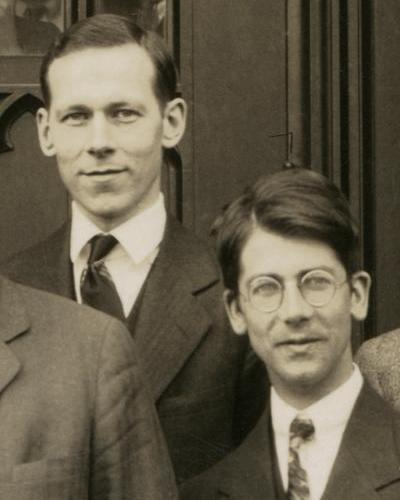
\includegraphics[width=\linewidth]{images/book3/mulliken-hund.jpg}
\end{minipage}\hfill
\begin{minipage}[t]{0.69\linewidth}
\vspace{0pt}
Entre 1926 e 1932, Friedrich Hund e Robert Mulliken interpretaram os espectros
das moléculas diatômicas atribuindo cada elétron a um orbital da molécula
inteira, classificado por sua simetria em torno do eixo. As palavras $\sigma$,
$\pi$, ligante e antiligante, e os diagramas de orbitais deste capítulo vêm de
seu trabalho; Mulliken recebeu o Prêmio Nobel de Química em 1966. A fotografia
mostra Mulliken (à esquerda) e Hund em Chicago, em 1929. (Fotografia: GFHund,
CC BY 3.0, Wikimedia Commons.)
\end{minipage}
\end{history}

\section{Ionização e força da ligação}

Retirar um elétron de um \omterm{def:b2:diatomic-mos:bonding}{orbital ligante} enfraquece a ligação; retirá-lo de
um \omterm{def:b2:diatomic-mos:bonding}{orbital antiligante} a fortalece. As energias de dissociação dos íons
decorrem de um ciclo termoquímico: para $\mathrm{AB}^+ \to \mathrm A + \mathrm B^+$,
\[
  D_0(\mathrm{AB}^+) = D_0(\mathrm{AB}) + I(\mathrm B) - I(\mathrm{AB}) ,
\]
sendo B o átomo de menor energia de ionização.

\begin{example}[Íons do nitrogênio e do oxigênio]\label{ex:b2:diatomic-mos:ions}
\ce{N2} ($I = \qty{15.58}{eV}$) perde um elétron ligante: $D_0(\ce{N2+}) = 9.76 + 14.53 -
15.58 = \qty{8.71}{eV}$, mais fraca que em \ce{N2}. \ce{O2} ($I = \qty{12.07}{eV}$) perde um
elétron $\pi^*$: $D_0(\ce{O2+}) = 5.12 + 13.62 - 12.07 = \qty{6.66}{eV}$, mais forte que em \ce{O2},
de acordo com as \omterm{def:b2:diatomic-mos:bond-order}{ordens de ligação} 2.5 e 2.5 contra 3 e 2.
% ledger: ie:N2, ie:N, ie:O2, ie:O, janafH0:N, janafH0:O
\end{example}

\section{Exercícios}

\begin{exercise}[$\star$]\label{exo:b2:diatomic-mos:1}
Para dois orbitais 1s do hidrogênio, tome $\alpha = \qty{-13.6}{eV}$, $\beta = \qty{-9.0}{eV}$ e
$S = 0.60$ (dados do exercício). Calcule $E_+$ e $E_-$ e depois a energia dos
dois elétrons de \ce{H2} comparada com dois átomos separados.
\end{exercise}

\begin{exercise}[$\star$]\label{exo:b2:diatomic-mos:2}
Dê as \omterm{def:b2:diatomic-mos:bond-order}{ordens de ligação} de \ce{He2}, \ce{He2+}, \ce{Li2} e \ce{B2} (com mistura
s--p).
\end{exercise}

\begin{exercise}[$\star$]\label{exo:b2:diatomic-mos:3}
Quais de \ce{B2}, \ce{C2}, \ce{N2}, \ce{O2}, \ce{F2} são \omterm{def:b2:diatomic-mos:magnetism}{paramagnéticas}?
\end{exercise}

\begin{exercise}[$\star$]\label{exo:b2:diatomic-mos:4}
O eixo molecular é $z$. Quais pares entre (1s, $2\mathrm p_z$), (1s,
$2\mathrm p_x$), ($2\mathrm p_x$, $2\mathrm p_x$), ($2\mathrm p_x$, $2\mathrm p_y$),
(2s, $2\mathrm p_z$) têm sobreposição não nula?
\end{exercise}

\begin{exercise}[$\star\star$]\label{exo:b2:diatomic-mos:5}
Preveja se \ce{N2+} tem uma ligação mais longa ou mais curta que \ce{N2} e
verifique com sua energia de dissociação calculada no capítulo.
\end{exercise}

\begin{exercise}[$\star\star$]\label{exo:b2:diatomic-mos:6}
O monóxido de carbono e \ce{N2} são isoeletrônicos. Explique por que os \omterm{def:b2:diatomic-mos:bonding}{orbitais
ligantes} de CO têm maior peso no oxigênio e por que seu orbital ocupado mais
alto é um par não ligante do carbono.
\end{exercise}

\begin{exercise}[$\star\star$]\label{exo:b2:diatomic-mos:7}
No HF, quais orbitais do flúor interagem com o 1s do hidrogênio, e quais
permanecem não ligantes? Desenhe o diagrama.
\end{exercise}

\begin{exercise}[$\star\star$]\label{exo:b2:diatomic-mos:8}
Com $\alpha_A = \qty{-10}{eV}$, $\alpha_B = \qty{-14}{eV}$ e $\beta = \qty{-3.0}{eV}$
(dados do exercício, $S$ desprezada), calcule as duas energias e o peso $c_B^2$
do \omterm{def:b2:diatomic-mos:bonding}{orbital ligante} em B.
\end{exercise}

\begin{exercise}[$\star\star$]\label{exo:b2:diatomic-mos:9}
Com mistura s--p, mostre que \ce{C2} tem \omterm{def:b2:diatomic-mos:bond-order}{ordem de ligação} 2, formada por duas
ligações $\pi$ e nenhuma ligação $\sigma_{2p}$.
\end{exercise}

\begin{exercise}[$\star\star\star$]\label{exo:b2:diatomic-mos:10}
Dê as \omterm{def:b2:diatomic-mos:bond-order}{ordens de ligação} de NO e de \ce{NO+}. A partir de $D_0(\ce{NO}) = \qty{6.51}{eV}$, $I(\ce{NO}) =
\qty{9.26}{eV}$ e $I(\ce{O}) = \qty{13.62}{eV}$, calcule $D_0(\ce{NO+})$ para $\ce{NO+} \to
\ce{N} + \ce{O+}$ e comente.
\end{exercise}

\begin{exercise}[$\star\star\star$]\label{exo:b2:diatomic-mos:11}
Mostre que $E_+ + E_- = 2(\alpha - \beta S)/(1 - S^2)$ e que essa soma supera $2\alpha$ quando
$\beta < \alpha S < 0$. Deduza por que dois orbitais preenchidos se repelem
(desestabilização a quatro elétrons).
\end{exercise}

\begin{exercise}[$\star\star\star$]\label{exo:b2:diatomic-mos:12}
Ordene \ce{O2+}, \ce{O2}, \ce{O2-}, \ce{O2^2-} por \omterm{def:b2:diatomic-mos:bond-order}{ordem de ligação}, comprimento
de ligação e força da ligação. Qual íon se encontra no peróxido de hidrogênio, e
qual no composto amarelo \ce{KO2}?
\end{exercise}

\section{Problema: O oxigênio e seus íons}

\begin{problem}[{Problema de fim de semana --- o diagrama de orbitais moleculares
do dioxigênio, as ordens de ligação e o magnetismo de seus íons, a ionização e
a força da ligação, e as duas maneiras de emparelhar os elétrons $\pi^*$}]
\label{pb:b2:diatomic-mos:1}
Dados: $I(\ce{O}) = \qty{13.62}{eV}$, $I(\ce{O2}) = \qty{12.07}{eV}$, $I(\ce{N}) =
\qty{14.53}{eV}$, $I(\ce{N2}) = \qty{15.58}{eV}$; $\Delta_f H_0$ a \qty{0}{K}
(\unit{kJ/mol}): \ce{O} 246.79, \ce{N} 470.82; $r_e$: \ce{O2} \qty{120.8}{pm}, \ce{N2}
\qty{109.8}{pm}; $1\ \unit{eV} = \qty{96.485}{kJ/mol}$.
% ledger: ie:O, ie:O2, ie:N, ie:N2, janafH0:O, janafH0:N, re:O2, re:N2

\medskip
\noindent\textbf{Parte I --- O dioxigênio.}
\begin{enumerate}
  \item Quantos elétrons de valência tem \ce{O2}?
  \item Desenhe seu diagrama de OM de valência (sem mistura s--p) e preencha-o.
  \item Calcule sua \omterm{def:b2:diatomic-mos:bond-order}{ordem de ligação}.
  \item Quantos elétrons desemparelhados? \ce{O2} é \omterm{def:b2:diatomic-mos:magnetism}{paramagnético}?
  \item Por que a estrutura de Lewis falha aqui?
  \item Calcule $D_0(\ce{O2})$ em \unit{eV}.
\end{enumerate}

\medskip
\noindent\textbf{Parte II --- Os íons.}
\begin{enumerate}[resume]
  \item Dê a configuração e a \omterm{def:b2:diatomic-mos:bond-order}{ordem de ligação} de \ce{O2+}.
  \item O mesmo para o íon superóxido \ce{O2-}.
  \item O mesmo para o íon peróxido \ce{O2^2-}.
  \item Dê o número de elétrons desemparelhados de cada íon.
  \item Ordene \ce{O2+}, \ce{O2}, \ce{O2-}, \ce{O2^2-} pelo comprimento de ligação previsto.
  \item Qual íon tem uma ligação simples O--O, como o peróxido de hidrogênio?
  \item Quais das quatro espécies são \omterm{def:b2:diatomic-mos:magnetism}{paramagnéticas}?
\end{enumerate}

\medskip
\noindent\textbf{Parte III --- A ionização.}
\begin{enumerate}[resume]
  \item De qual orbital sai o elétron quando \ce{O2} é ionizado?
  \item Por que $I(\ce{O2})$ é menor que $I(\ce{O})$?
  \item Mostre que $D_0(\ce{O2+}) = D_0(\ce{O2}) + I(\ce{O}) - I(\ce{O2})$ e calcule-a.
  \item Compare com $D_0(\ce{O2})$ e explique.
  \item Calcule $D_0(\ce{N2})$ e $D_0(\ce{N2+})$ da mesma maneira.
  \item Por que $I(\ce{N2})$ é maior que $I(\ce{N})$?
  \item Resuma: quando a ionização fortalece uma ligação?
\end{enumerate}

\medskip
\noindent\textbf{Parte IV --- Os elétrons $\pi^*$.}
\begin{enumerate}[resume]
  \item No estado fundamental, os dois elétrons $\pi^*$ ocupam dois orbitais
        diferentes com spins paralelos. Que regra diz isso?
  \item Descreva um estado no qual ambos ocupam o mesmo orbital $\pi^*$.
  \item Por que esse estado é mais alto em energia?
  \item Quais são sua \omterm{def:b2:diatomic-mos:bond-order}{ordem de ligação} e seu magnetismo?
  \item Dê a \omterm{def:b2:diatomic-mos:bond-order}{ordem de ligação} de \ce{O2+} e sua energia de dissociação.
\end{enumerate}
\end{problem}
